% !TEX root = mythesis.tex

%==============================================================================
\chapter{Data Analysis}
\label{sec:data_analysis}
%==============================================================================
\section{Image Visual Inspection}
\section{Surface Brightness Analysis}
\subsection{Full Azimuthal Surface Brightness Analysis}
\begin{figure}[htbp]
    \centering
    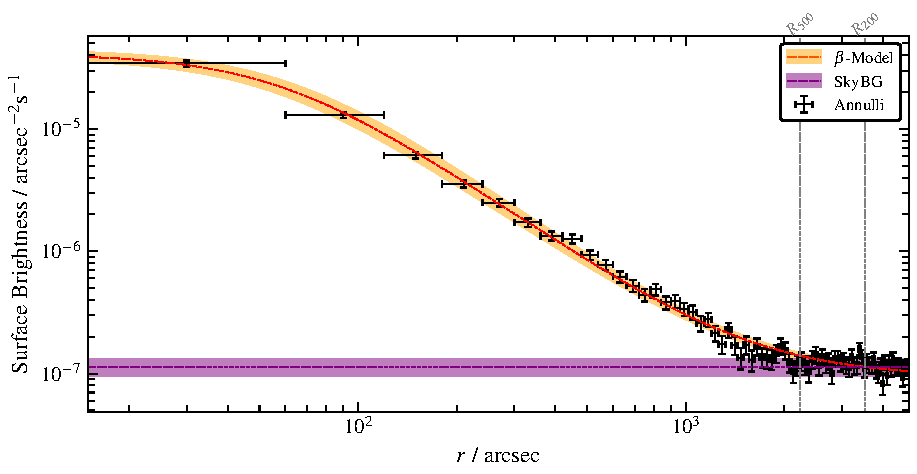
\includegraphics{data_analysis/beta_model_tot_surf_bri_anulli1_1arcmin.pdf}
    \caption{A nice plot.}
\end{figure}
To accurately quantify potential asymmetries in the X-ray emission of NGC 1550, surface brightness analysis is performed. First, the emission center is estimated by constructing a \(2'\) aperture around the apparent center, as given in Section X. This aperture size is chosen to capture a statistically significant number of photons while minimizing bias from potential asymmetries outside the group center. The flux-weighted average of the image coordinates within this aperture yields a right ascension of \SI{64.909}{\degree} and a declination of \SI{2.414}{\degree}. Concentric Anulli with \(1'\) width are constructed from the calculated flux-weighted surface brightness of the group up to \(80'\). The counts \(C\) within each annulus are determined using the \texttt{funcnts} task from the \texttt{funtools} software, with a Poisson error of \(\sqrt{C}\). The surface brightness \(S\) for each annulus is calculated by
\begin{align*}
    S = \frac{C_\text{image} - C_\text{PIB}}{C_\text{expmap}\cdot A},
\end{align*}
where \(C\) denotes the counts in the photon image, total PIB map, and exposure map, respectively. Errors are calculated using Gaussian error propagation. Furthermore,background estimation is performed using \(10\) circular regions with a \(48'\) radius, each centered \(160'\) from the calculated center of NGC 1550. The average background surface brightness is evaluated for all circles combined and separately for the northern (Circles 1-5) and southern regions (Circles 6-10) to account for possible background gradients. 
